\section{Spacecraft Control Architecture Rapid Simulator (SCARS) Toolbox}\label{sec:toolbox}
% This chapter describes the top-level architecture of the
\textit{Short description of the chapter.}

\textit{What SCARS means and what it is.}

\textit{Describe briefly what is the input and the output of the whole toolbox.}

%todo: add Navigation Toolbox to Software choice.

\subsection{Objectives}\label{toolbox:objectives}

    \begin{itemize}
        \item Provide model of orbital dynamics of Earth orbiting satellite;
        \item Create models of most common satellite actuators and sensors and parametrize them so that actual hardware can be reproduced in simulation using parameters from datasheets;
        \item Include sources of environmental forces and torques, modeling most influential sources;
        \item Implement several of the most basic control methods;
        \item Create a Simulink Custom Library, with all models masked for quick set up;
        \item Provide methods of conducting preliminary review of feasibility of used hardware components and control methods;
        \item Create interfaces allowing the user to connect the toolbox with visualization software;
    \end{itemize}

\subsection{Choice of software}
    To fit with the objectives of accessibility and ease of modification MATLAB family of software was chosen. MATLAB is one of the most popular scripting language and with the addition of Simulink software it can become powerful tool with the ability to set up numerical simulations in short time. MATLAB is taught in most technical universities and there is significant number of both courses available online and materials for self-teaching. For one purpose (described in Section \ref{sec:ksp}) a Python script acting as a dataflow bridge was used, as it was a simplest method to solve a problem described in that chapter. Several other software solutions were used for visualization purposes, with the reasoning described in \autoref{sec:visualization}.

    Versatility of MATLAB is often attributed to the number of Add-Ons available for it. \ac{scars} Toolbox uses and requires the following modules:
    \begin{itemize}
        \item Aerospace Toolbox
        \item \dots
        \item \dots
    \end{itemize}
    
    %todo: cite courses and tutorials

\subsection{Architecture}
    \ac{scars} is divided into two parts: 1) Parts Library and 2) Modular Simulation. The Parts Library contains Simulink subsystems, which can be connected to form simulations of various complexity and for multiple scenarios. The other is a Modular Simulation, which can be set up with either MATLAB command line scripts or graphical user interface.

    \subsubsection{Parts Library}
        %TODO: Should I write something about the aim of the library?
        \ac{scars} Parts Library is a ready to use Simulink Custom Library, that is a collection of blocks available to use in Simulink models. All blocks in library downloaded alongside \ac{scars} are parametrized, masked and described to ease the integration of library parts into user simulation. The library is divided into specific sections:
        \begin{itemize}
            \item Satellite Dynamics
            \item Reference Frames Transformations
            \item Environment
            \item Actuators
            \item Sensors
            \item Control Algorithms
            \item Visualization
            \item Analysis
            \item Examples
        \end{itemize}

        \begin{figure}[H]
            \centering
            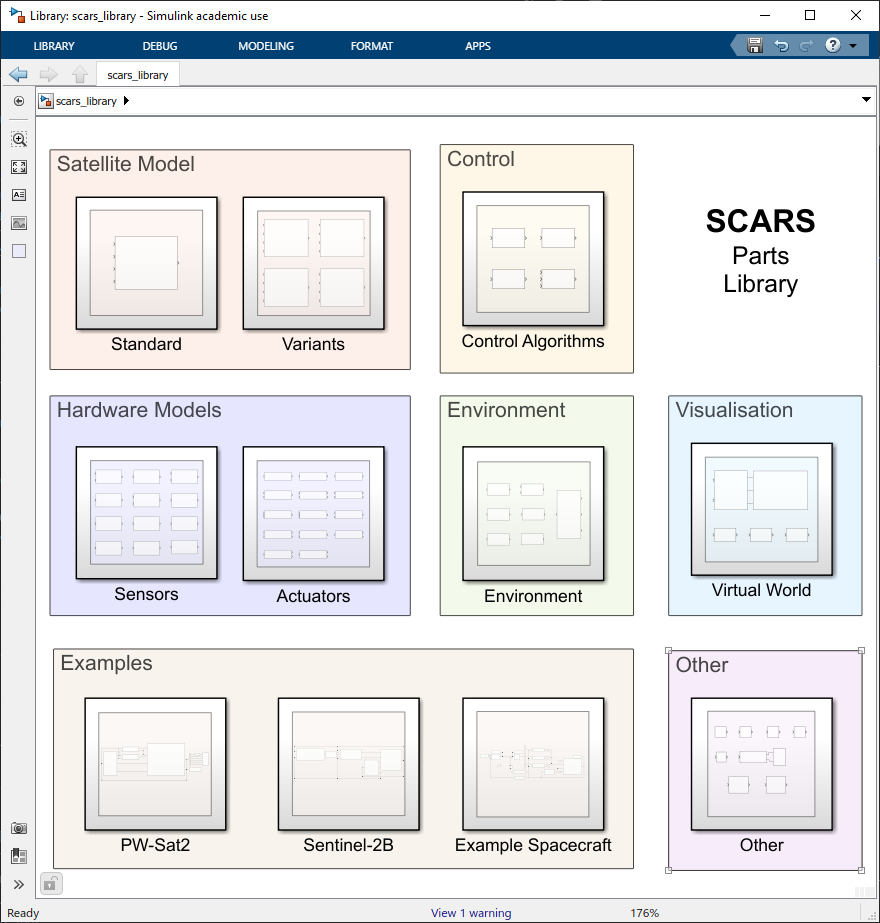
\includegraphics[width=1\textwidth]{2-toolbox/scars-library.png}
            \caption{SCARS Parts Library screenshot}
            \label{fig:scars-library}
        \end{figure}

    \subsubsection{Modular Simulation}
        \ac{scars} Modular Simulation is a ready-made simulink model available for setup using prepared scripts and \ac{scars} user interface. The model is a simulation of cube-shaped satellite, which can be set on specified orbit using various initialization methods, such as Keplerian elements in conjunction with Julian date time. (The initialization is further described in Chapter \ref{sec:documentation}). In the same manner, all actuators and sensors available in \ac{scars} library can be chosen. The Modular Simulation makes use of most available blocks, which can be commented out from the model, either by hand or using the user interface, to improve the speed of the simulation.

        \begin{figure}[H]
            \centering
            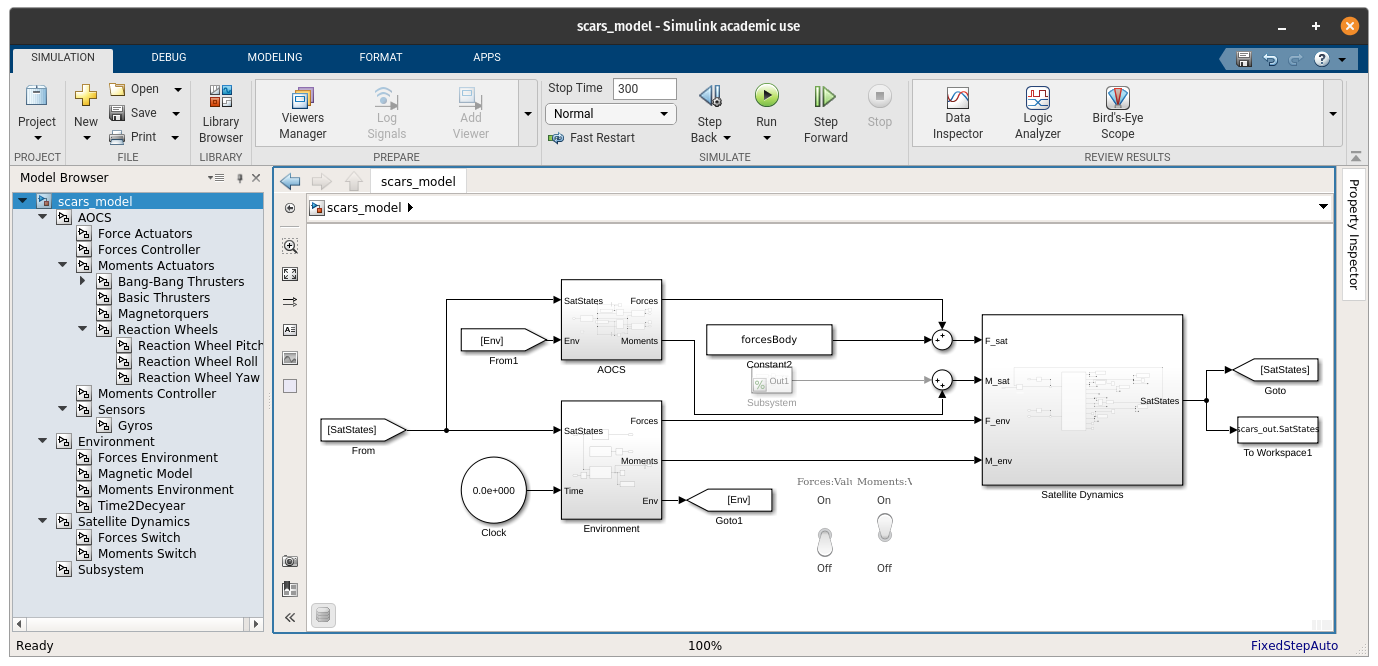
\includegraphics[width=1\textwidth]{2-toolbox/scars-model.png}
            \caption{SCARS Modular Simulation screenshot}
            \label{fig:scars-model}
        \end{figure}
